\chapter{Badania platformy}
\label{chapter:research}

Badania systemu służą do sprawdzenia wpływu zastosowania platformy na wykonanie projektu, w~tym ocenę usprawnienia pracy studentów i~zmiany ich sposobu uczestnictwa w~projekcie.
Dodatkowo badania narzędzia pozwoliły na ocenę łatwości i~intuicyjności obsługi interfejsów oraz ocenę zadowolenia użytkowników z~działania platformy.

Aby zbadać platformę przeprowadzono symulację dwóch hipotetycznych projektów.
Dla obu zadań grupa testowa od początku zna pełny cel każdego z~nich.
Wykonywanie kolejnych etapów przybliża uczestników do pełnej realizacji zadania.
Taki typ projektu jest bardzo często prowadzony w~ramach różnych przedmiotów na wydziale EiTI.

Oba zadania zostały przeprowadzone na grupie testowej, składającej się z~absolwentów Politechniki Warszawskiej.
Opis motywów doboru członków grupy testowej znajduje się w~podrozdziale \ref{research_group}.

Pierwsza z~symulacji jest przeprowadzeniem projektu podobnego do historycznego zadania wykonywanego przez studentów w~semestrze zima 2018 w~ramach przedmiotu ”Podstawy Programowania”.
Pełna definicja problemu, przebieg symulacji oraz wnioski zostały przedstawione w~podrozdziale \ref{research_penguins}.

Drugie zadanie sprowadza się do napisania programu pozwalającego na wykonywanie operacji matematycznych na macierzach.
Ma ono na celu zbadanie użyteczności tworzenia procesów integracji programów w~ramach platformy.
Opis tej symulacji znajduje się w~podrozdziale \ref{research_matrix}.

Kolejny podrozdział zawiera wnioski z~nadania absolwentom uprawnień administratora podczas testowania platformy.
Okazało się, że bardzo chętnie tworzyli oni własne etapy i~testowali swój kod przy użyciu narzędzia.
Doprowadziło to do wniosku, że platforma mogłaby zostać rozszerzona w~przyszłości (nie tracąc dotychczasowych funkcjonalności) tak, aby możliwe było również przeprowadzenie z~jej użyciem projektów w~metodyce Agile.

Ostatni podrozdział \ref{research_summary} zawiera podsumowanie przeprowadzonych badań.


\section{Opis grupy testowej}
\label{research_group}

W skład grupy testowej, na której zostały przeprowadzone obie symulacje projektów, wchodziło dwóch absolwentów Politechniki Warszawskiej.
Obie osoby ukończyły wydział Elektroniki i~Technik Informacyjnych.

Absolwenci brali udział w~projektach grupowych realizowanych na wydziale EiTI i~znają podstawy programowania.
Dzięki temu mają pełne zaplecze wiedzy potrzebnej do realizacji każdego z~symulowanych projektów.
Mogą oni dzięki swojemu doświadczeniu ocenić czy zastosowanie platformy byłoby użyteczne podczas prowadzenia projektów studenckich.
Absolwenci potrafią także wskazać różnice w~prowadzeniu projektu bez użycia platformy oraz z~jej wykorzystaniem.

Obie osoby posiadają również doświadczenie komercyjne, dzięki temu są w~stanie ocenić narzędzie od strony technicznej i~zasugerować dodatkowe funkcjonalności mające na celu zwiększenie użyteczności platformy.

Drugą rozpatrywaną grupą osób, która mogłaby wydawać się właściwa do przetestowania użyteczności platformy są obecni studenci.
Taki pomysł zespołu testowego został jednak odrzucony ze względu na ciągły proces udoskonalania narzędzia podczas badań.

W testowanej wersji MVP mogą wystąpić nieprzewidziane zachowania platformy.
Wynika to z~faktu, że w~początkowej fazie projektu ciężko jest wyeliminować wszystkie błędy.
Do ich całkowitego usunięcia trzeba utrzymywać i~wspierać aplikację na bieżąco.
Takie niewielkie problemy pojawiły się podczas badania platformy przez grupę absolwentów i~były na bieżąco naprawiane.

Udostępnienie studentom platformy bez przetestowania jej na mniejszej grupie mogłoby spowodować rezultat odwrotny do zamierzonego.
Zamiast wykorzystać zalety rozwiązania takie osoby mogłyby zniechęcić się ze względu na występujące błędy.
Sam czas naprawy błędów mógłby nie być satysfakcjonujący dla studentów i~pogłębiać frustrację.
W przypadku studentów pierwszego roku przekazanie narzędzia na takim etapie pracy zdecydowanie utrudniłoby im wykonanie projektu.

Warto również zaznaczyć, że studenci zwłaszcza pierwszego roku nie mają szerokiego doświadczenia w~uczestnictwie w~projektach grupowych.
Stąd wprowadzenie dodatkowych narzędzi mogłoby wzbudzać u nich początkową niechęć.
Mogłoby okazać się, że dopiero po zebraniu większego doświadczenia właściwie oceniliby wpływ platformy na proces ich pracy.

Przekazanie platformy w~obecnej wersji dla studentów i~monitorowanie ich interakcji z~platformą podczas pełnego projektu jest jedną ze wskazanych możliwości kontynuacji pracy.
Dzięki analizie przebiegu rzeczywistego projektu uczelnianego można byłoby zrozumieć lepiej proces pracy studentów i~uzupełnić platformę o~dodatkowe, pożyteczne funkcjonalności.


\section{Symulacja zmodyfikowanego projektu historycznego}
\label{research_penguins}

Do zdefiniowania zadania dla symulacji projektu historycznego posłużono się projektem wykonywanym przez studentów w~ramach przedmiotu ”Podstawy Programowania” w~realizacji zima 2018.
Jest to ten sam typ zadania, który posłużył do weryfikacji platformy.

Przeprowadzenie symulacji sprowadza się do następujących kroków:
\begin{enumerate}
    \item Analiza i~przedefiniowanie treści projektu.
    \item Utworzenie projektu na platformie.
    \item Udostępnienie projektu grupie testowej.
    \item Analiza wykonanej pracy przez absolwentów i~sformułowanie wniosków.
\end{enumerate}

Aby umożliwić przetestowanie aplikacji poprzez testy akceptacyjne zmodyfikowano treść historycznego zadania i~zakres kolejnych etapów.
W podrozdziale \ref{penguins_project_definition} opisano definicję projektu, która posłużyła do przeprowadzenia symulacji.

Kolejna sekcja \ref{penguins_simulation} opisuje przebieg symulacji dla projektu historycznego.

W ramach ostatniego podrozdziału zamieszczono analizę wykonanej pracy przez absolwentów.
Opisano również wnioski z~eksperymentu.


\subsection{Definicja projektu wraz z~przypadkami testowymi}
\label{penguins_project_definition}

Do definicji projektu posłużono się historycznym zadaniem wykonywanym przez studentów w~ramach przedmiotu ”Podstawy Programowania”.
Pełna definicja historycznego projektu znajduje się w~załączniku.

Niestety historyczne założenia projektowe nie umożliwiały wykorzystania w~pełni potencjału automatyzacji wprowadzanego przez platformę.
Nie pozwalały one między innymi na przetestowanie aplikacji poprzez testy akceptacyjne zarówno w~wersji iteraktywnej, jak i~w~wersji AI.
Dokładana analiza problemów związanych z~bezpośrednim użyciem historycznych założeń projektowych została opisana w~poprzednim rozdziale \ref{chapter:verify}.
W ramach badania zmodyfikowano założenia i~zakres kolejnych etapów, tak aby uzyskać korzyści z~przeprowadzenia projektu z~wykorzystaniem platformy.

W ramach symulacji projektu na platformie zostały utworzone trzy etapy.
Celem kolejnych zadań jest:
\begin{enumerate}
    \item Wczytanie i~walidacja planszy.
    \item Ustawienie pingwina na wskazanym polu planszy.
    \item Wykonanie zadanego ruchu pingwinem.
\end{enumerate}

Dla każdego z~etapów zarówno plik wejściowy, jak i~wyjściowy posiada ten sam format jak w~definicji historycznego projektu.
Zmianie uległy przyjmowane przez aplikacje parametry wykonania.


W ramach pierwszego etapu utworzono dwa przypadki testowe sprawdzające:
\begin{itemize}
    \item poprawność walidacji pliku wejściowego,
    \item czy w~przypadku poprawnie zdefiniowanej planszy jest ona wypisywana do pliku wyjściowego.
\end{itemize}
Do definicji przypadków testowych dla pierwszego etapu nie użyto żadnych dodatkowych parametrów.
Wejściowe oraz oczekiwane wyjściowe pliki dla powyższych testów zostały zamieszczone w~załącznikach.


Dla drugiego etapu stworzono cztery przypadki testowe.
Jeden z~przypadków ocenia czy aplikacja poprawnie ustawia pingwina na dozwolonym polu.
Pozostałe trzy testy sprawdzają zachowanie programu dla przypadków brzegowych takich, jak:
\begin{itemize}
    \item próba ustawienia pingwina na polu ze zbyt dużą liczbą ryb,
    \item próba ustawienia pingwina poza planszą,
    \item próba ustawienia gracza, który nie istnieje dla danej rozgrywki.
\end{itemize}

Do definicji akcji ustawiania pingwina dla drugiego etapu użyto czterech parametrów:
\begin{itemize}
    \item \textit{id=i}, gdzie \textit{i} jest identyfikatorem gracza i~przyjmuje wartość od 1 do 9,
    \item \textit{phase=placement}, gdzie \textit{placement} oznacza fazę rozmieszczania,
    \item \textit{placement\_x=j}, gdzie \textit{j} przyjmuje wartość od 0 do n-1 i~oznacza położenie pingwina w~poziomie,
    \item \textit{placement\_y=k}, gdzie \textit{k} przyjmuje wartość od 0 do m-1 i~oznacza położenie pingwina w~pionie.
\end{itemize}

Dla trzeciego etapu stworzono trzy przypadki testowe.
Jeden z~testów ocenia czy program poprawnie przemieszcza pingwina na dozwolone pole.
Inne dwa przypadki testowe sprawdzają zachowanie aplikacji dla warunków brzegowych, takich jak:
\begin{itemize}
    \item próba przesunięcia pingwina na pole, na którym znajduje się inny pionek,
    \item próba przemieszczenia pingwina poza planszę.
\end{itemize}

Do definicji akcji przesunięcia pingwina dla trzeciego etapu użyto pięciu parametrów:
\begin{itemize}
    \item \textit{id=i}, gdzie \textit{i} jest identyfikatorem gracza i~przyjmuje wartość od 1 do 9,
    \item \textit{phase=move}, gdzie \textit{move} oznacza fazę ruchu,
    \item \textit{from\_x=j}, gdzie \textit{j} przyjmuje wartość od 0 do n-1 i~oznacza początkowe położenie pingwina w~poziomie,
    \item \textit{from\_y=k}, gdzie \textit{k} przyjmuje wartość od 0 do m-1 i~oznacza początkowe położenie pingwina w~pionie,
    \item \textit{direction=d}, gdzie \textit{d} przyjmuje jedną z~wartość: \textit{up, down, left, right} i~oznacza kierunek przesunięcia pingwina.
\end{itemize}

Plik zawierające dane dla testów utworzonych dla wszystkich trzech etapów zostały zamieszczone w~załącznikach.

Dla projektu utworzono również jeden proces integracji z~pojedynczym testem akceptacyjnym.
Proces składał się z~dwóch kroków, kolejno: \textit{set} i~\textit{move}.
Utworzony test akceptacyjny pozwolił na sprawdzenie pozytywnego przebiegu akcji ustawienia a następnie przesunięcia pingwina.

\subsection{Przebieg symulacji}
\label{penguins_simulation}
Już na samym początku symulacji zmodyfikowane zadanie okazało się proste do implementacji i~trudne do podziału pomiędzy członków zespołu.
Z tych powodów projekt samodzielnie wykonał jeden absolwent.

W ramach symulacji absolwentowi został udostępniony historyczny opis projektu oraz zmodyfikowany zakres przyjmowanych parametrów dla zadania.
Następnie poproszono go o~zalogowanie się do platformy przy użyciu własnego konta GitHub.

Symulacja była na bieżąco monitorowana.
W trakcie jej trwania poprawiano definicję projektu.
Między innymi zdecydowano się uzupełnić etap pierwszy i~drugi o~dodatkowe przypadki testowe, które sprawdzały warunki brzegowe.

Już po kilku pierwszych iteracjach absolwent wyraził zadowolenie z~korzystania z~narzędzia.
W~trakcie wykonywania zadania dodał, że ułatwia ono mu pracę a dzięki zdefiniowanym przypadkom testowym może skupić się na implementacji logiki aplikacji.

W tabelach od \ref{tab:read_parse_write} do \ref{tab:move_penguins} przedstawiono pełne historie uruchomień programów dla wszystkich trzech etapów w~ramach symulacji.

\begin{table}[H]
    \centering
    \caption{Historia uruchomienia programu dla etapu \textit{Read parse write}.}
\scalebox{0.8}{
\begin{tabular}{|l|l|l|l|l|}
    \hline
    \rowcolor[HTML]{EFEFEF}
    \textbf{Próba}  & \textbf{Data} & \textbf{Użytkownik} & \textbf{Nazwa testu} & \textbf{Status} \\ \hline
    1 &     Sat Aug 17 13:00:57 CEST 2019        & first\_user@mail.com            &                                             &                                        \\ \hline
    &       &                                            & Read parse write                            & FAILURE                                \\ \hline
    2 &     Sat Aug 17 13:05:18 CEST 2019        & first\_user@mail.com            &                                             &                                        \\ \hline
    &       &                                            & Read parse write                            & FAILURE                                \\ \hline
    3 &     Sat Aug 17 13:10:52 CEST 2019        & first\_user@mail.com            &                                             &                                        \\ \hline
    &       &                                            & Read parse write                            & FAILURE                                \\ \hline
    4 &     Sat Aug 17 13:12:40 CEST 2019        & first\_user@mail.com            &                                             &                                        \\ \hline
    &       &                                            & Read parse write                            & FAILURE                                \\ \hline
    5 &     Sat Aug 17 13:13:32 CEST 2019        & first\_user@mail.com            &                                             &                                        \\ \hline
    &       &                                            & Read parse write                            & SUCCESS                                \\ \hline
    6 &     Sat Aug 17 14:54:13 CEST 2019        & first\_user@mail.com            &                                             &                                        \\ \hline
    &       &                                            & Read parse write                            & SUCCESS                                \\ \hline
    7 &     Sat Aug 17 15:00:24 CEST 2019        & first\_user@mail.com            &                                             &                                        \\ \hline
    &       &                                            & Read parse write                            & SUCCESS                                \\ \hline
    8 &      Sat Aug 17 15:09:38 CEST 2019        & first\_user@mail.com            &                                             &                                        \\ \hline
    &       &                                            & Read parse write                            & FAILURE                                \\ \hline
    9 &     Sat Aug 17 15:11:13 CEST 2019        & first\_user@mail.com            &                                             &                                        \\ \hline
    &       &                                            & Read parse write                            & SUCCESS                                \\ \hline
    10 &    Sat Aug 17 15:16:42 CEST 2019        & first\_user@mail.com            &                                             &                                        \\ \hline
    &       &                                            & Read parse write                            & SUCCESS                                \\ \hline
    11 &    Sat Aug 17 18:16:11 CEST 2019        & first\_user@mail.com            &                                             &                                        \\ \hline
    &       &                                            & Invalid input file                          & FAILURE                                \\ \hline
    &       &                                            & Read parse write                            & SUCCESS                                \\ \hline
    12 &    Sat Aug 17 18:30:40 CEST 2019        & first\_user@mail.com            &                                             &                                        \\ \hline
    &       &                                            & Invalid input file                          & FAILURE                                \\ \hline
    &       &                                            & Read parse write                            & SUCCESS                                \\ \hline
    13 &    Sat Aug 17 18:31:47 CEST 2019        & first\_user@mail.com            &                                             &                                        \\ \hline
    &       &                                            & Invalid input file                          & SUCCESS                                \\ \hline
    &       &                                            & Read parse write                            & SUCCESS                                \\ \hline
\end{tabular}
\label{tab:read_parse_write}

}
\end{table}


%\begin{table}[]
%    \label{tab:set_penguins}
%\centering
%\caption{Statystyki dla etapu \textit{Set penguins}}
\scriptsize
\begin{center}
%\scalebox{0.7}{
    \begin{longtable}{|l|l|l|l|}
        \caption{Statystyki dla etapu \textit{Set penguins}}
        \label{tab:set_penguins} \\\hline
        %
        \hline
        \rowcolor[HTML]{EFEFEF}
        \textbf{Data}                 & \textbf{Użytkownik}             & \textbf{Nazwa testu}             & \textbf{Status} \\ \hline
        Sat Aug 17 17:52:24 CEST 2019 & chcialemmiecinnylogin@gmail.com &                                  &                 \\ \hline
        &                                 & Place player 2 on 3 4            & FAILURE         \\ \hline
        Sat Aug 17 17:54:27 CEST 2019 & chcialemmiecinnylogin@gmail.com &                                  &                 \\ \hline
        &                                 & Place player 2 on 3 4            & FAILURE         \\ \hline
        Sat Aug 17 17:54:46 CEST 2019 & chcialemmiecinnylogin@gmail.com &                                  &                 \\ \hline
        &                                 & Place player 2 on 3 4            & FAILURE         \\ \hline
        Sat Aug 17 17:58:23 CEST 2019 & chcialemmiecinnylogin@gmail.com &                                  &                 \\ \hline
        &                                 & Place player 2 on 3 4            & FAILURE         \\ \hline
        Sat Aug 17 18:08:04 CEST 2019 & chcialemmiecinnylogin@gmail.com &                                  &                 \\ \hline
        &                                 & Place player 2 on 3 4            & FAILURE         \\ \hline
        Sat Aug 17 18:08:10 CEST 2019 & chcialemmiecinnylogin@gmail.com &                                  &                 \\ \hline
        &                                 & Place player 2 on 3 4            & FAILURE         \\ \hline
        Sat Aug 17 18:08:35 CEST 2019 & chcialemmiecinnylogin@gmail.com &                                  &                 \\ \hline
        &                                 & Place player 2 on 3 4            & SUCCESS         \\ \hline
        Sat Aug 17 18:35:19 CEST 2019 & chcialemmiecinnylogin@gmail.com &                                  &                 \\ \hline
        &                                 & Place player 2 on 3 4            & SUCCESS         \\ \hline
        &                                 & Place on cell with too many fish & FAILURE         \\ \hline
        &                                 & Place outside of board           & FAILURE         \\ \hline
        &                                 & Place with player id too high    & FAILURE         \\ \hline
        Sat Aug 17 18:35:38 CEST 2019 & chcialemmiecinnylogin@gmail.com &                                  &                 \\ \hline
        &                                 & Place player 2 on 3 4            & SUCCESS         \\ \hline
        &                                 & Place on cell with too many fish & FAILURE         \\ \hline
        &                                 & Place outside of board           & FAILURE         \\ \hline
        &                                 & Place with player id too high    & FAILURE         \\ \hline
        Sat Aug 17 18:40:24 CEST 2019 & chcialemmiecinnylogin@gmail.com &                                  &                 \\ \hline
        &                                 & Place player 2 on 3 4            & SUCCESS         \\ \hline
        &                                 & Place on cell with too many fish & FAILURE         \\ \hline
        &                                 & Place outside of board           & FAILURE         \\ \hline
        &                                 & Place with player id too high    & FAILURE         \\ \hline
        Sat Aug 17 18:42:48 CEST 2019 & chcialemmiecinnylogin@gmail.com &                                  &                 \\ \hline
        &                                 & Place player 2 on 3 4            & SUCCESS         \\ \hline
        &                                 & Place on cell with too many fish & FAILURE         \\ \hline
        &                                 & Place outside of board           & FAILURE         \\ \hline
        &                                 & Place with player id too high    & FAILURE         \\ \hline
        Sat Aug 17 18:46:00 CEST 2019 & chcialemmiecinnylogin@gmail.com &                                  &                 \\ \hline
        &                                 & Place player 2 on 3 4            & SUCCESS         \\ \hline
        &                                 & Place on cell with too many fish & FAILURE         \\ \hline
        &                                 & Place outside of board           & FAILURE         \\ \hline
        &                                 & Place with player id too high    & FAILURE         \\ \hline
        Sat Aug 17 18:46:13 CEST 2019 & chcialemmiecinnylogin@gmail.com &                                  &                 \\ \hline
        &                                 & Place player 2 on 3 4            & FAILURE         \\ \hline
        &                                 & Place on cell with too many fish & SUCCESS         \\ \hline
        &                                 & Place outside of board           & SUCCESS         \\ \hline
        &                                 & Place with player id too high    & FAILURE         \\ \hline
        Sat Aug 17 18:47:45 CEST 2019 & chcialemmiecinnylogin@gmail.com &                                  &                 \\ \hline
        &                                 & Place player 2 on 3 4            & SUCCESS         \\ \hline
        &                                 & Place on cell with too many fish & FAILURE         \\ \hline
        &                                 & Place outside of board           & SUCCESS         \\ \hline
        &                                 & Place with player id too high    & SUCCESS         \\ \hline
        Sat Aug 17 18:49:02 CEST 2019 & chcialemmiecinnylogin@gmail.com &                                  &                 \\ \hline
        &                                 & Place player 2 on 3 4            & FAILURE         \\ \hline
        &                                 & Place on cell with too many fish & FAILURE         \\ \hline
        &                                 & Place outside of board           & SUCCESS         \\ \hline
        &                                 & Place with player id too high    & SUCCESS         \\ \hline
        Sat Aug 17 18:52:01 CEST 2019 & chcialemmiecinnylogin@gmail.com &                                  &                 \\ \hline
        &                                 & Place player 2 on 3 4            & SUCCESS         \\ \hline
        &                                 & Place on cell with too many fish & SUCCESS         \\ \hline
        &                                 & Place outside of board           & SUCCESS         \\ \hline
        &                                 & Place with player id too high    & SUCCESS         \\ \hline
    \end{longtable}
%}
\end{center}
%\end{table}

\normalsize


\begin{table}[H]

\centering
\caption{Historia uruchomienia programu dla etapu \textit{Move penguins}}
\scalebox{0.65}{
\begin{tabular}{|l|l|l|l|l|}
    \hline
    \rowcolor[HTML]{EFEFEF}
    \textbf{Próba}  & \textbf{Data}                 & \textbf{Użytkownik}                   & \textbf{Nazwa testu}                     & \textbf{Status} \\ \hline
    1 &             Sat Aug 17 20:17:55 CEST 2019 & first\_user@mail.com &                                        &                 \\ \hline
    &               &                                 & Move penguin 1 1 down to other penguin & FAILURE         \\ \hline
    &               &                                 & Move penguin 1 1 up                    & SUCCESS         \\ \hline
    &               &                                 & Move penguin 1 3 right to empty        & SUCCESS         \\ \hline
    2 &             Sat Aug 17 20:22:25 CEST 2019 & first\_user@mail.com &                                        &                 \\ \hline
    &               &                                 & Move penguin 1 1 down to other penguin & FAILURE         \\ \hline
    &               &                                 & Move penguin 1 1 up                    & SUCCESS         \\ \hline
    &               &                                 & Move penguin 3 1 right to empty        & FAILURE         \\ \hline
    3 &             Sat Aug 17 20:23:38 CEST 2019 & first\_user@mail.com &                                        &                 \\ \hline
    &               &                                 & Move penguin 1 1 down to other penguin & SUCCESS         \\ \hline
    &               &                                 & Move penguin 1 1 up                    & SUCCESS         \\ \hline
    &               &                                 & Move penguin 3 1 right to empty        & SUCCESS         \\ \hline
\end{tabular}
\label{tab:move_penguins}
}
\end{table}

Powyższe statystyki nie zawieraja komunikatów o~błędzie, które są również zapisywane przez platformę.
Dodanie ich pogorszyłoby znacznie czytelność tabel, ze względu na za dużą ilość informacji.

Na podstawie powyższych historii uruchomień programów można stwierdzić, że absolwent wykonywał etapy kolejno.
Nie tworzył on od razu pełnej logiki aplikacji.
Kod był pisany przez niego inkrementacyjnie.
Programy pisane w~ramach poszczególnych etapów były uruchamiane przez niego regularnie.
Widać również, że zmieniając logikę aplikacji doprowadzał do regresji kodu.

W ramach etapu drugiego zostało wykonane najwięcej iteracji.
To zadanie wymagało zaimplementowania logiki umieszczania pingwina wraz z~uwzględnieniem warunków brzegowych.
Ostatni etap wymagał od absolwenta zrealizowania tylko trzech iteracji.
Dla tego zadania logika aplikacji była juz w~większości zaimplementowana i~zatwierdzona w~ramach poprzednich etapów.

Proces integracji został uruchomiony raz, po poprawnym ukończeniu ostatniego etapu i~zakończył się sukcesem.

Na rysunku \ref{fig:penguins_simulation_interface} przedstawiony został wynik symulacji z~perspektywy prowadzącego.

\begin{figure}[h]
    \centering
    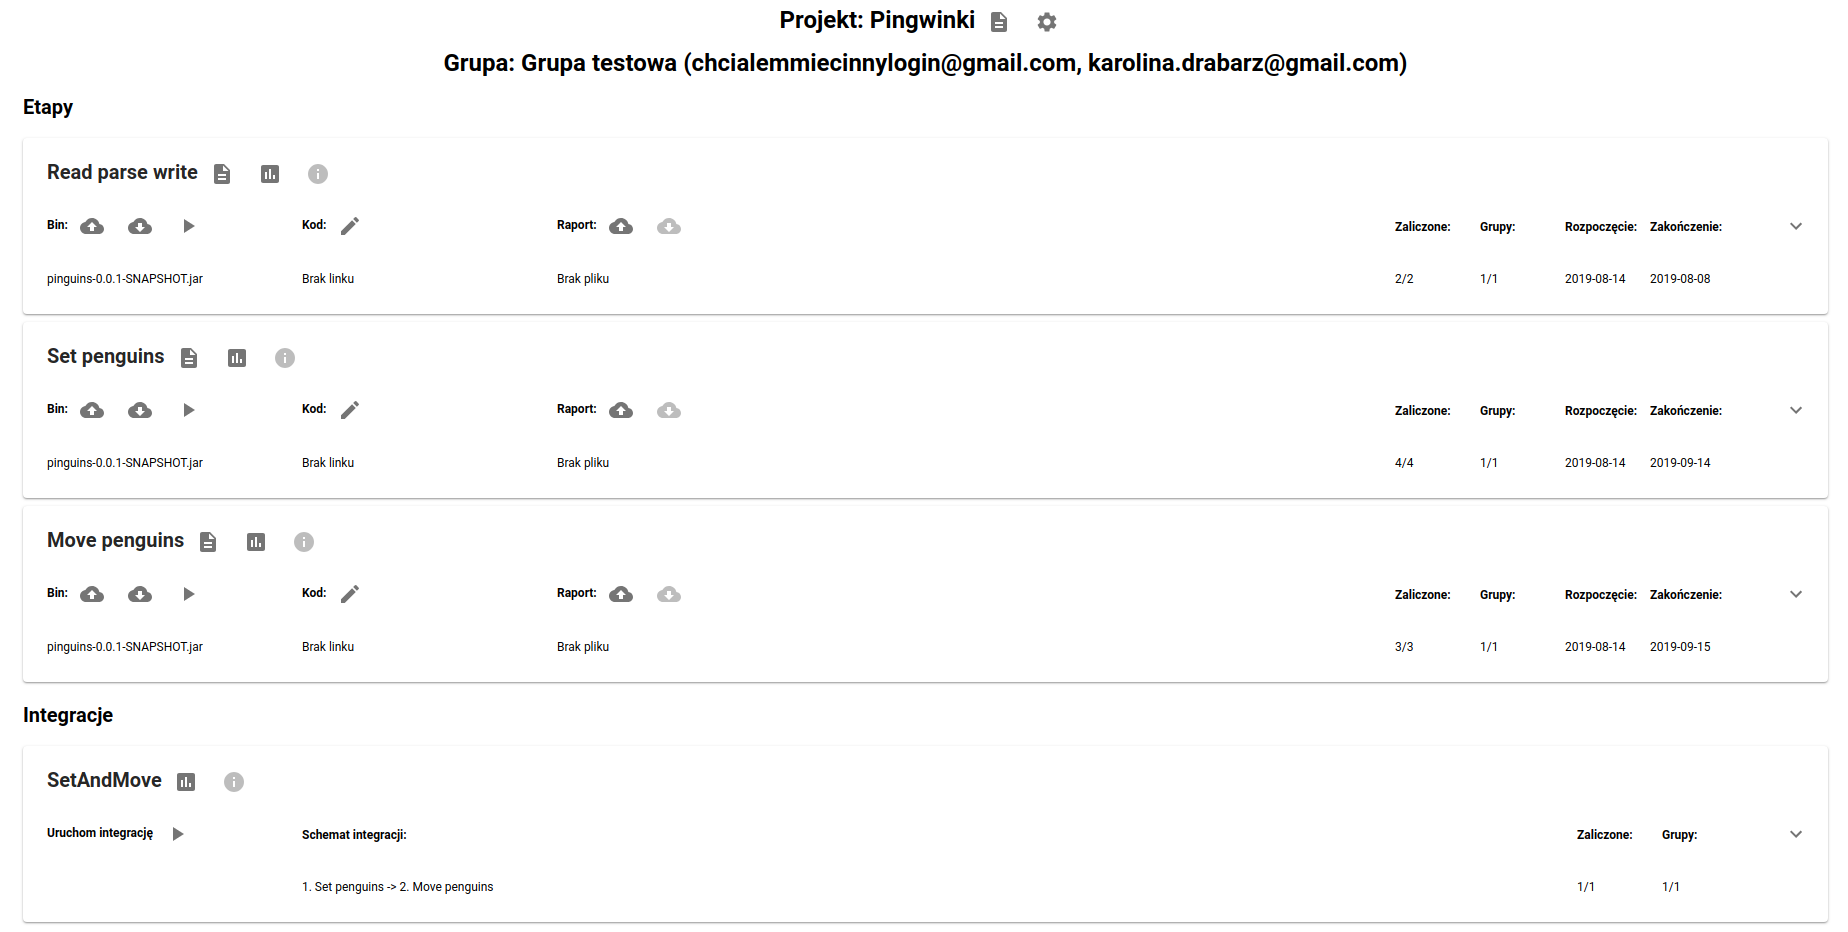
\includegraphics[width = 16cm]{chapter07/penguins_preview.png}
    \caption{Podgląd postępów studentów w~ramach symulacji zmodyfikowanego projektu historycznego.}
    \label{fig:penguins_simulation_interface}
\end{figure}


\subsection{Podsumowanie}

Platforma została oceniona pozytywnie.
Podczas symulacji nie wystąpiły znaczące problemy z~jej użytkowaniem.
Oferowany przez narzędzie interfejs graficzny był intuicyjny, czytelny i~zrozumiały.

Po ukończeniu projektu absolwent uznał, że zadanie zostało podzielone we właściwy i~jasny sposób na kolejne etapy.
Testy akceptacyjne były dobrze dobrane i~pozwoliły na przetestowanie wartości brzegowych.

Sam kod był pisany przez absolwenta inkrementacyjnie.
Programy były wielokrotnie uruchamiane na platformie i~sprawdzany był wynik ich wykonania.
Absolwent był zadowolony z~uzyskanej informacji zwrotnej.
Również czas, po jakim otrzymywał ją był dla niego akceptowalny.
Dodatkowo platforma pozwoliła na wykrycie regresji dla kolejnych wersji programów.
Potwierdza to użyteczność platformy od strony studenta.

Proces tworzenia programu był na bieżąco monitorowany.
Podczas symulacji zmodyfikowano projekt dodając dodatkowe przypadki testowe.
Aby uniknąć takiej sytuacji w~przypadku prawdziwego projektu studenckiego zalecane jest, żeby prowadzący tworząc kolejne etapy na bieżąco tworzył własny program testowy i~sprawdzał poprawność definicji testów akceptacyjnych.
Wcześniejsze doświadczenie w~pracy z~wybranym do realizacji projektem wydaje się być również kliczowe, na pewno pozwoliłoby zminimalizować przykładowo ewentualne niespójności w~definicji kolejnych etapów i~integracji.

Dla pierwszego etapu dopiero dodanie przypadku testowego oczekującego na wypisanie komunikatu o~błędzie w~przypadku niepoprawnego formatu pliku wejściowego wymusiło na absolwencie napisanie pełnej i~poprawnej implementacji kodu do parsowania planszy.
Absolwent uznał, że po dodaniu drugiego testu etap był bardzo dobrze zdefiniowany.
Implementacja poprawnego parsownia planszy sprawiła, że ilość pracy potrzebnej do zrealizowania kolejnych zadań stała się wyważona.
Ten fakt podkreśla istotę odpowiedniego doboru testów akceptacyjnych dla etapów.

Rezultaty wykonania kolejnych etapów są przekazane w~jasny sposób na interfejsie platformy.
Dzięki temu można bardzo szybko ocenić postępy pracy.
W~przypadku symulacji, wymagana logika programu napisanego przez absolwenta dla każdego z~etapów była poprawna, ponieważ testy akceptacyjne załączone do projektu zostały wykonane pomyślnie.
Statystyki z~uruchomienia aplikacji pokazują, że absolwent z~zaangażowaniem wykonywał kolejne zadania.

Przeprowadzona integracja przebiegła pomyślnie.
Oznacza to, że programy napisane w~ramach kolejnych etapów używały spójnego formatu danych.
Definicja testów akceptacyjnych na platformie wymusiła jednakowy protokół przekazywania informacji.
W~przypadku gdy w~ramach projektu uczestniczyłoby więcej grup projektowych programy, które pomyślnie przeszłyby kolejne etapy również używałyby spójnego formatu danych, przez co można byłoby wykonać pomyślną próbę integracji aplikacji pomiędzy zespołami.

\section{Symulacja projektu z~procesem integracji}
\label{research_matrix}

Drugi typ symulacji ma na celu zbadanie użyteczności zaimplementowanego w~ramach platformy procesu integracji.
Wykonanie pełnego zadania projektowego sprowadza się do napisania aplikacji pozwalającej na wykonywanie określonych operacji matematycznych na macierzach.

Proces tej symulacji można podzielić na następujące kroki:
\begin{enumerate}
    \item Definicja treści projektu.
    \item Utworzenie projektu na platformie.
    \item Udostępnienie projektu grupie testowej.
    \item Analiza wykonanej pracy przez absolwentów i~sformułowanie wniosków.
\end{enumerate}

W podrozdziale \ref{matrix_project_definition} opisano definicję symulowanego projektu.
Kolejna sekcja \ref{matrix_simulation} opisuje przebieg zadania wykonanego przez grupę testową.
W ramach ostatniego podrozdziału przeanalizowano i~podsumowano badanie.


\subsection{Definicja projektu wraz z~przypadkami testowymi}
\label{matrix_project_definition}

W ramach symulacji projektu na platformie zostało utworzone pięć etapów.
Celem kolejnych zadań jest:
\begin{enumerate}
    \item Mnożenie macierzy przez skalar.
    \item Dodanie macierzy.
    \item Transpozycja macierzy.
    \item Rotacja macierzy o~90 stopni zgodnie z~ruchem wskazówek zegara (rotacja w~prawo o~90 stopni).
    \item Mnożenie dwóch macierzy.
\end{enumerate}

W ramach każdego etapu utworzono cztery przypadki testowe sprawdzające poprawność działań.
Plik wejściowy opisuje macierz o~rozmiarze n na m i~jest takiego samego formatu dla każdego z~zadań.
Zawiera on m wierszy, gdzie w~każdym z~nich znajduje się n liczb oddzielonych spacją reprezentujących elementy macierzy.
Wspomniane cztery przypadki testowe przyjmują w~pliku wejściowym macierze o~kolejnych rozmiarach: 2 na 2, 2 na 3, 3 na 2 oraz 3 na 3.

Oprócz pliku wejściowego zawierającego definicję macierzy część testów przyjmuje również parametry wejściowe.
W przypadku pierwszego etapu parametrem wejściowym jest pojedyncza liczba reprezentująca skalar.
Program wykonujący drugi oraz piąty etap powinien przyjmować jako parametr wejściowy drugą macierz.
Format opisujący macierz zawartą w~pliku z~parametrami dla zadania cztery i~pięć jest taki sam jak format pliku wejściowego.
Dla trzeciego i~czwartego zadania niepodawane są parametry wejściowe.

Oprócz testów sprawdzających poprawność wykonania działań zdefiniowano również przypadki sprawdzające czy walidacja danych wejściowych jest prawidłowa.
Dla wszystkich etapów utworzono pojedyncze testy sprawdzające poprawność formatu pliku wejściowego.
Dodatkowe dwa przypadki testowe, sprawdzające poprawność formatu pliku z~parametrami oraz rozmiary obu wejściowych macierzy zostały dodane dla etapu drugiego oraz piątego.

Pliki zawierające dane dla wszystkich powyższych testów zostały zamieszczone w~załącznikach.

TODO: Opisać definicje integracji

\subsection{Przebieg symulacji}
\label{matrix_simulation}

TODO: Opisać


\subsection{Podsumowanie}

TODO: Napisać


\section{Udostępnienie grupie testowej platformy z~prawami administratora}

W celu pełnego i~dokładnego przetestowania zaimplementowanej platformy udostępniono ją członkom grupy testowej z~nadanymi prawami administratora.
Ten rodzaj testów odbył się dodatkowo, poza opisanymi wcześniej badaniami.
Dzięki nadaniu praw administratora studenci mogli sami tworzyć i~definiować projekty.
W wyniku ich testów można było wychwycić nieprawidłowości w~działaniu platformy oraz ocenić intuicyjność i~łatwość obsługi interfejsów prowadzącego.
Pozwoliło to również na określenie czy integracja interfejsów z~serwerem jest właściwa.

W wyniku tych testów okazało się, że absolwenci bardzo chętnie definiowali własne projekty, etapy i~integracje.
Z zaangażowaniem dodawali oni przypadki testowe i~tworzyli programy spełniające założenia kolejnych zadań.

Analiza aktywności grupy testowej po udostępnieniu jej narzędzia z~rolą administratora doprowadziła do wniosku, że platforma mogłaby zostać użyta nie tylko do polepszenia procesu weryfikacji pracy studentów podczas standardowego projektu informatycznego.
Narzędzie mogłoby również posłużyć monitorowaniu prac studentów dla projektu prowadzonego w~metodyce Agile.
W związku z~możliwością użycia platformy również dla takiego typu zadania w~ramach pracy dokonano zgrubnej analizy przeprowadzenia tego typu projektu.

W podrozdziale \ref{agile_proposition} omówiono propozycję przeprowadzenia zwinnego projektu.
Sekcja opisuje \ref{agile_todo} podstawowe funkcjonalności, jakie należałoby zaimplementować w~kolejnej wersji platformy tak, aby była ona użyteczna w~prowadzeniu projektów w~metodyce Agile.
Ostatni podrozdział zawiera krótkie podsumowanie.

\subsection{Propozycja przeprowadzenia zwinnego projektu z~użyciem platformy}
\label{agile_proposition}

Dla projektu prowadzonego w~metodyce Agile na początku semestru studenci dostawaliby luźno zdefiniowany, ogólny cel pracy.
W trakcie semestru ich zadaniem byłoby doprecyzowanie z~prowadzącym szczegółów.
Dla takiego podejścia prowadzący traktowany byłby jako PO (ang. Product Owner), z~którym studenci odbywaliby regularne spotkania.

Studenci w~ramach takiego projektu sami decydowaliby o~wyznaczeniu kolejnych zadań oraz raportowali o~statusie ich wykonania.
Do tego procesu mogłaby posłużyć zmodyfikowana platforma, umożliwiająca studentom definicję własnego projektu.
Zdaniem grupy byłoby samodzielne stworzenie kolejnych etapów wraz z~poszerzeniem wiedzy na temat projektu.
Dla każdego z~kolejnych zadań studenci mieliby za zadanie napisać własne testy akceptacyjne.
Dzięki wykorzystaniu platformy prowadzący miałby możliwość podejrzenia wyników prac poszczególnych grup w~dowolnym momencie.

W przypadku zwinnej metodyki nawet dla takiego samego początkowego celu projektu dla każdej z~grup, wyniki pracy w~ciągu semestru będą różne.
Z tego powodu wydaje się, że pełne indywidualne podejście i~rozważenie postępów dla każdego z~zespołów jest nieuniknione.
W rzeczywistości można by było jednak ograniczyć i~zautomatyzować ocenę poczynań studentów poprzez wykorzystanie platformy.
Tak jak w~przypadku tradycyjnego projektu, tak samo dla zadania prowadzonego w~metodyce Agile prowadzący miałby jednolity wgląd w~postępy studentów.
Kolejne etapy byłyby definiowane przez studentów w~analogiczny sposób w~ramach każdego z~projektów.
Informacje opisujące kolejne zadania wyświetlane byłyby przy użyciu tego samego interfejsu niezależnie od projektu czy grupy.
Prowadzący na pierwszy rzut oka mógłby łatwo ocenić postępy prac w~ramach jedno zespołu czy nawet wstępnie porównać zaangażowanie w~projekt pomiędzy dwoma zespołami.

Jak zostało wyjaśnione wcześniej, napisane przez studentów testy akceptacyjne mogą nie dawać wysokiego pokrycia.
Ocena słuszności przypadków testowych przez prowadzącego jest czasochłonna.
Dzięki użyciu platformy prowadzący miałby wgląd do testów na wysokim poziomie.
Aby zrozumieć przypadek testowy, nie musiałby on bezepośrednio przeglądać kodu studentów.
Jego zadanie sprowadzałoby się do zrozumienia zawartości pliku wejściowego, oczekiwanego pliku wyjściowego i~parametrów.
Ocena testów byłaby wciąż indywidaulna, ale tu również dla każdego projektu prezentowane byłyby one w~ten sam sposób.

\subsection{Dodatkowe funkcjonalności wymagające implementacji}
\label{agile_todo}

Osiągnięcie przedstawionych w~poprzednim podrozdziale celów nie jest możliwe przy użyciu platformy w~obecnej wersji MVP i~wymagałoby dokonania kilku modyfikacji w~ramach narzędzia.
W celu wskazania pełnych zmodyfikowanych założeń projektowych należałoby przeanalizować dokładnie problemy stojące za przeprowadzeniem projektu w~metodyce Agile.
W ramach pracy przeprowadzono zgrubną analizę takiego podejścia i~wskazano główne modyfikacje, jakich należałoby dokonać w~narzędziu.

Jedną z~podstawowych zmian jest dodatnie dodatkowego poziomu uprawnień.
Obecnie w~ramach platformy istnieją tylko dwie role: prowadzącego (administratora) oraz studenta (zwykłego użytkownika).
W modelu MVP zakłada się, że w~ramach platformy może istnieć kilku prowadzących, którzy mają dostęp do edycji każdego z~projektów, ale pomimo takich uprawnień ich zachowanie jest odpowiedzialne i~nie edytują oni projektów innych niż własne.
Dla zwinnego projektu należałoby umożliwić wskazanej grupie studentów zarządzanie pojedynczym projektem.
Wymagałoby to dodatkowej roli w~bazie posiadającej szersze uprawnienia niż zwykły student.
Warto jednak zauważyć, że dodatkowe uprawnienia nie powinny być równe z~prawami administratora, który ma między innymi możliwość usunięcia całego projektu.
W celu odpowiedniej definicji nowej roli i~zakresu jej uprawnień należałoby przeanalizować dokładniej problem.

Ważnym zagadnieniem jest również równoległy dostęp platformy.
Dla obecnej wersji narzędzia jedyna akcja, dla której wymagane jest strzeżenie równoległego dostępu to uruchamianie programów.
Łatwo zauważyć, że w~przypadku zwinnego projektu, również definiowanie etapów i~integracji mogłoby wymagać równoległego dostępu do zasobów.
Dodatkową funkcjonalnością byłoby dodanie obserwacji zmian dokonywanych na platformie w~ramach projektu i~aktualizacji interfejsów studentów podążających za tymi zmianami.

W przypadku zwinnego projektu zbierane statystyki powinny być szersze niż dla tradycyjnego podejścia.
Dla wersji MVP przechowywane są one tylko dla uruchomień kolejnych programów.
W wersji podstawowej zakłada się, że prowadzący zna wymagania i~definiuje projekt na początku semestru, po czym udostępnia go studentom.
Może on dokonywać modyfikacji zadań w~trakcie trwania semestru, jednak z~założenia nie powinny być one duże.
W przypadku gdy studenci sami mieliby zarządzać projektem należałoby, zbierać również informacje dotyczące tworzenia zadań i~przechowywać je nawet dla usuniętych etapów i~integracji.
Takie informacje pozwoliłyby na lepsze zrozumienie specyfiki pracy studentów w~przypadku zwinnego projektu.
Mogłyby posłużyć również do oceny pracy semestralnej i~porównania zaangażowania w~obrębie różnych zespołów.

Inną wartą rozważenia funkcjonalnością jest dodanie komentarza dla tworzonych przez studentów przypadków testowych.
Pomimo takiego samego przedstawienia testów w~ramach wszystkich projektów ich ocena byłaby dalej indywidualna.
Jest to czasochłonne i~kłopotliwe.
Dodanie dodatkowego komentarza dla każdego z~testów mogłoby być przydatne do lepszego zrozumienia zamiarów studentów w~przypadku bardziej złożonych przypadków testowych.

Kolejną przydatną funkcjonalnością jest możliwość zatwierdzania etapów przez prowadzącego.
Zaakceptowanie powinno odbywać się po spotkaniu z~prowadzącym, jednak taka funkcjonalność mogłaby dodatkowo pomóc w~ocenie końcowej przebiegu projektu.

Wszystkie omówione modyfikacje można wprowadzić do platformy, nie tracąc przy tym jej dotychczasowych funkcjonalności.
W większości nie są to trudne do zaimplementowania zmiany, jednak wymagają one przed wprowadzeniem dodatkowej, pełniejszej analizy.
Dodanie nowej roli i~wprowadzenie pełniejszego zrównoleglenia dostępu do zasobów powinno być dobrze przemyślane i~zaprojektowane przed implementacją.

\subsection{Podsumowanie}

Platforma może zostać rozszerzona, tak aby możliwe było z~jej wykorzystaniem przeprowadzenie zwinnego projektu.
Modyfikacje nie powinny wpłynąć na obecne funkcjonalności platformy.
Dzięki takiemu podejściu narzędzie stałoby się jeszcze bardziej uniwersalne.

Pomysł udostępnienia platformy dla zwinnych projektów nasunął się podczas badania gotowego narzędzia.
Był to moment, w~którym platforma została zweryfikowana w~podstawowej wersji.
Dodanie na tym etapie pracy nowych funkcjonalności mogłoby doprowadzić do destabilizacji platformy i~nie przyniosłoby pozytywnych rezultatów.
Stąd udostępnienie platformy do prowadzenia projektów w~metodyce Agile jest proponowanym rozszerzeniem pracy magisterskiej.


\section{Podsumowanie}
\label{research_summary}

TODO:
Z badań powinno wynikać zrealizowanie założeń -
na marginesie, jakie są założenia pracy (możliwość stworzenia środowiska opierającego się na samoocenie, przez co proces weryfikacji po stronie prowadzącego znacznie się upraszcza).
Nie jestem pewna, czy to na pewno wyłania się obecnie z~podsumowania.

TODO: Coś więcej napisać o~Agile, dodać matrix (eee czy na pewno?)

- być może nie powinni również móc usuwać etapów które zostały przedstawione i~zatwierdzone w~jakiś sposób przez prowadzącego??

- można rozszerzyć o~projekty Agile i~wtedy platforma staje sie super uniwersalnym narzędziem

- jak tworzy się przypadki testowe to na bieżąco trzeba tworzyć binarkę i~sprawdzać (prowadzący musi robić swoją - tak najwygodniej)

- zaczyna się od testów i~przemyślenia ich (platforma troche to narzuca od strony prowadzącego)

- najlepiej przemyslec calosciowa koncepcje

- potem krok po kroku dodawac etapy i~testy i~po dodaniu etapow i~testow dodac binarke

- ale zawsze mozna dodac tez jakis test pozniej i~przedefiniowac zadanie

- wychodzi takie pseudo TDD (przynajmniej dla prowadzacego, studenci moga dalej nie umiec pisac testow i~zrobic i~tak zle testy na koniec)

- wygodne narzedzie, wlasciwie testy byly napisane wiec grupa testowa skupila sie na rozwiazaniu problemu

- wielokrotnie odpalali binarki

- poprawiali bledy

- widac bylo regresje

- wazne jest zeby dobrze zdefiniowac przypadki testowe

- bardzo dobrze ze przypadki testowe sa udostepnione stuentom

- dzieki udostepnienieniu przypadkow moga oni w~latwy sposob ocenic i~rozumiec co jest nie tak

- najlepiej dodac wlasny komparator dla miedzy innymi niestabilnych algorytmów

- obecny komparator porownuje dwa pliki 1 do 1 i~moze sluzyc do definicji wiekszosci zadan

- ale może okazać sie ze to zbyt mało

- po zbadaniu platformy doszly zmiany funkcjonalnosci (niewielkie) ulatwiajace prace

- okazalo sie ze platforma jest intuicyjna i~pomocna

- testy na wysokim poziomie - latwe do zrozumienia

- testy nie blokuja implementacji co jest bardzo wazne

- nie ma znaczenia jak w~srodku studenci napisza program, testy nie wymuszaja implementacji



